\chapter{Direkte Fernlokalisierung mit LoRa}
\label{ch:phase4}
Für die direkte Fernlokalisierung mit LoRa werden dedizierte Basisstationen eingesetzt. 
Die Kommunikation zwischen Basisstation und Ortungsserver kann durch ein LAN- oder WLAN-Netzwerk gewährleistet werden.
Die Basisstationen bestimmen des Received Signal Strength Index eingehender Übertragungen der mobilen Enheiten und übermitteln die gemessenen Werte dann an den Ortungsserver.
Der Ortungsserver kann mit den gesammelten Werten die Position der mobilen Einheit berechnen.

\section{RFM95}
\label{ch:hardwarechanges:sec:rfm95}
Bei dem RFM95 handelt es sich um ein LoRa (Long Range) fähiges Radio-Modul für den Frequenzbereich 868/915MHz \cite{hope2006rfm}. 
915MHz sind jedoch nur in Amerika lizenzfrei, in Deutschland muss das Radio mit 868MHz betrieben werden.\\
Für die Entwicklung wird das Modul auf einem Adafruit Feather M0 RFM95 LoRa Radio verwendet.
Dieses verwendet zusätzlich einen M0 Mikrocontroller zur Steuerung, einen Lithium-Akku-Ladeschaltkreis und einen Spannungswandler zur einfachen Programmierung des Radios über USB.
Zusätzlich ist eine Antenne notwendig, die verwendete Antenne kann dabei einen große Unterschiede in der Reichweite verursachen, deshalb sollte eine Antenne für 868MHz verwendet werden.
Da jedoch eine feste Antenne die mobile Einheit unhandlich machen würde, wird für diese eine Kabelantenne verwendet, diese hat die Länge einer halben Wellenlänge (17,3cm).\\
Abbildung \ref{fig:lorafeather} zeigt zwei Feather M0 RFM95 LoRa Radio. 
Das RFM95 mit Kabelantenne dient als mobile Einheit und das RFM95 mit fester Antenne dient als Basisstation.

\begin{figure}[h]
  \centering
	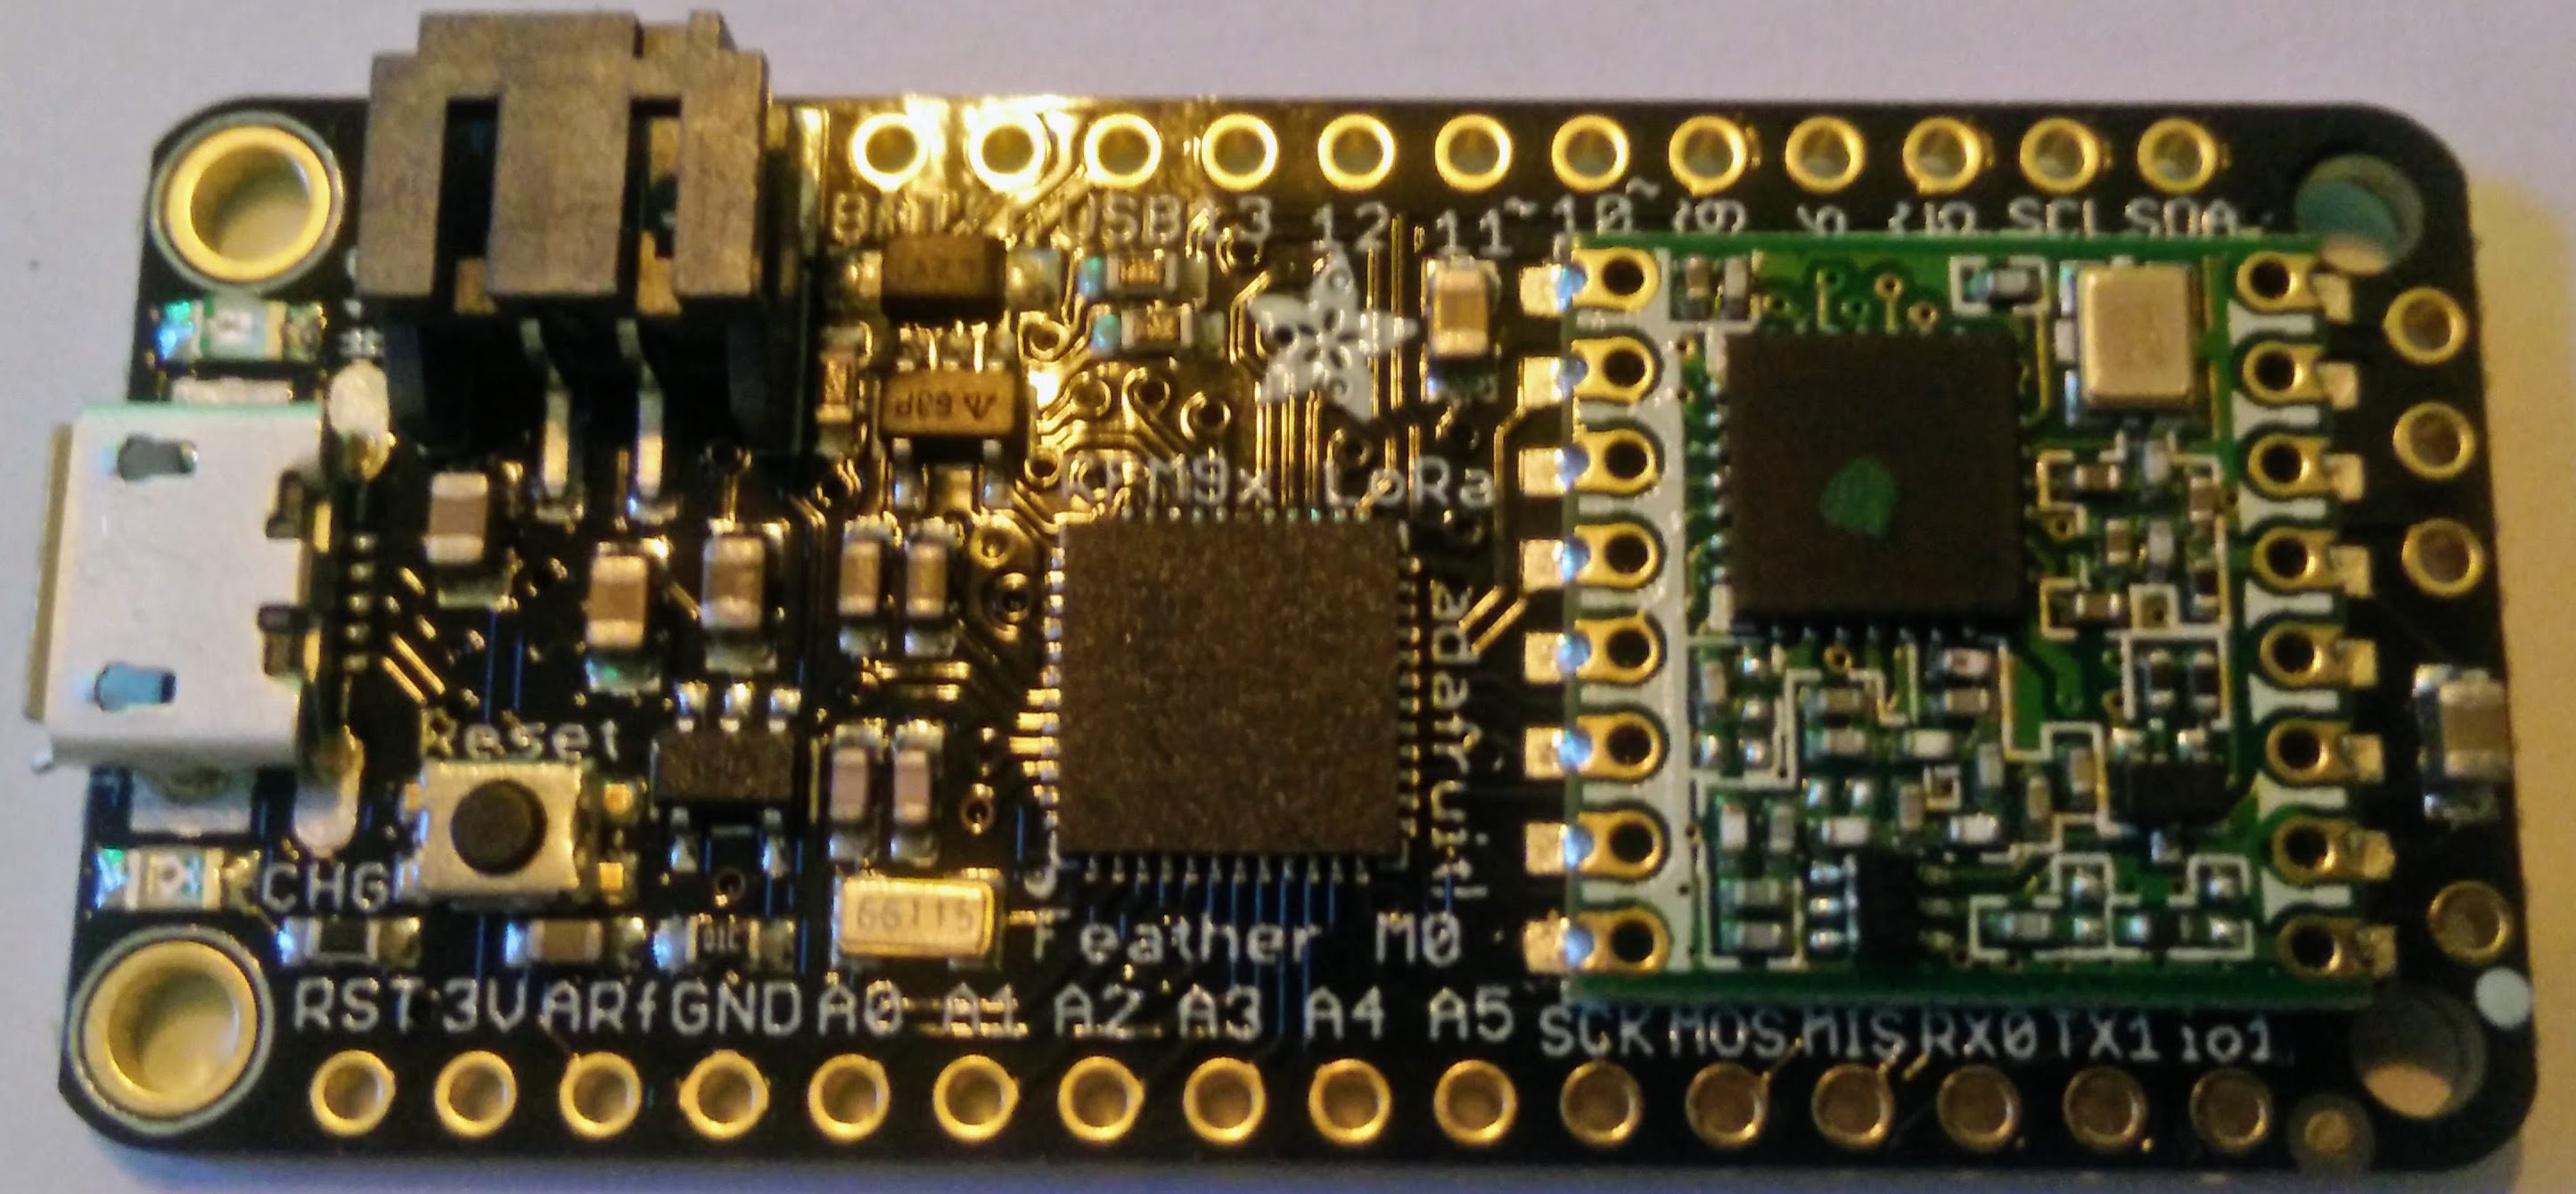
\includegraphics[width=\textwidth]{images/lorafeather.jpg}
  \caption{Adafruit LoRa Feather mit RFM95}
  \label{fig:lorafeather}
\end{figure}

\subsection{RadioHead RFM9x für Arduino}
Der M0 Mikrocontroller ist Arduino kompatibel, wird zusätzlich die RadioHead RFM9x Bibliothek verwendet, kann er über ein SPI-Interface das Radio steuern.
Dazu muss zunächst in den Optionen der Arduino IDE unter \textit{Additional Boards Manager URLs} die URL \url{https://adafruit.github.io/arduino-board-index/package_adafruit_index.json} hinzugefügt werden \cite{treece2016lora}.
Nach einem Neustart der IDE können im \textit{Board Manager} die \texttt{Arduino SAMD Boards} installiert werden. 
Der M0 kann nun programmiert werden, um das RFM95 verwenden zu können muss die RadioHead RFM9x Bibliothek von \url{https://cdn-learn.adafruit.com/assets/assets/000/035/106/original/RadioHead-1.62.zip} heruntergeladen und nach \\\texttt{/Arduino/libraries/} entpackt werden.

\section{Reichweite von LoRa}
Die Versuche mit LoRa wurden an einer anderen Tunnelbaustelle durchgeführt.
An der Tunnelbohrstelle Ulm wird mit Sprengungen vorgetrieben.
Nach der Sprengung wird der Tunnel mit Spritzbeton ausgekleidet und danach wird in drei Schritten geschalt. 
Im ersten Schritt wird ein Filz und eine Folie gegen das Eindringen von Wasser eingebracht, danach folgt die Bewehrung und abschließend wird die Bewehrung einbetoniert.
Für jeden Schritt wird ein stählerner Schalungswagen verwendet, folglich sind drei stählerne Hindernisse im Tunnel, die Signale absorbieren.
Abbildung \ref{fig:schalungswagen} zeigt einen der Schalungswagen, der als Hindernis gedient hat.

\begin{figure}[h]
  \centering
	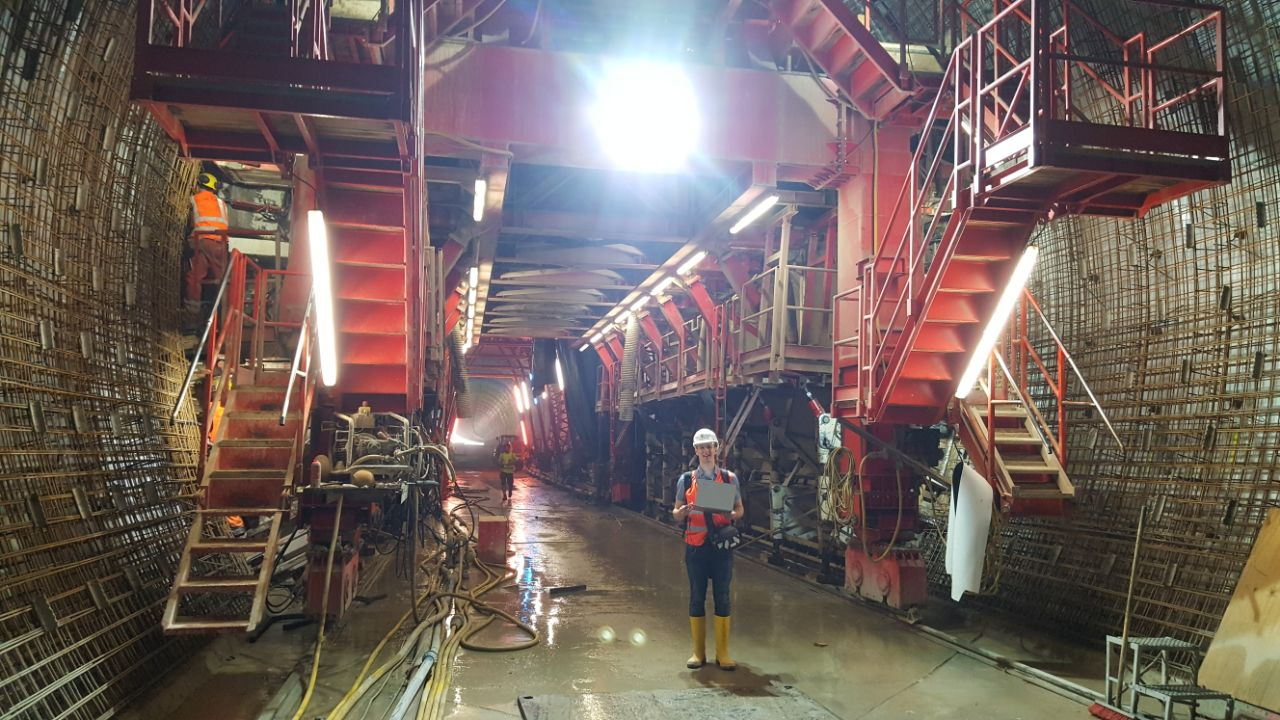
\includegraphics[width=\textwidth]{images/schalungswagen.jpg}
  \caption{Schalungswagen für das Betonieren im Tunnel Ulm.}
  \label{fig:schalungswagen}
\end{figure}

\subsection{Methodik} 
Die Reichweite wurde für zwei Situationen bestimmt.
Zum einen durch einen Schalungswagen und dann durch den freien Tunnel, zum anderen durch alle drei Schalungswagen für eine Situation mit maximaler Abschirmung durch die Hindernisse.
Die mobile Einheit wurde jeweils direkt an der Bewehrung platziert und es wurde auf der selben Seite gelaufen, damit die Abschirmung durch die Schalungswagen maximal ist.
Danach wurde die Basisstation immer weiter entfernt, bis keine Pakete der mobilen Einheit mehr empfangen werden konnten.
Abbildung \ref{fig:lorabasis} zeigt die Platzierung der mobilen Einheit an der Bewehrung.
Erneut konnte die Plastikbox aufgrund des Versuchsaufbaus nicht geschlossen werden.
Die mobile Einheit wurde als "{}außer Reichweite"{} angesehen, wenn versendete Pakete der mobilen Einheit nicht mehr bei der Basisstation ankamen.
Durch das Entfernen des körperlichen Hindernisses war es möglich wieder eine Verbindung herzustellen.
Es wurde sowohl mit einer Sendeleistung von 5dBm für einen geringen Sendeverbrauch als auch mit 23dBm Sendeleistung für maximale Reichweite gemessen.
Die Messungen werden in 12,5 Meter Abständen angegeben, da in diesem Tunnel die Länge eines Schalungselements 12,5 Meter beträgt.
Es werden, wie in Abschnitt \ref{ch:hardwarechanges:sec:rfm95} besprochen, zwei unterscheidliche Typen von Antennen verwendet. 
Während die Basisstation eine feste Antenne aufweist, verwendet die mobile Einheit eine Kabelantenne entsprechend der halben Wellenlänge. 

\begin{figure}[h]
  \centering
	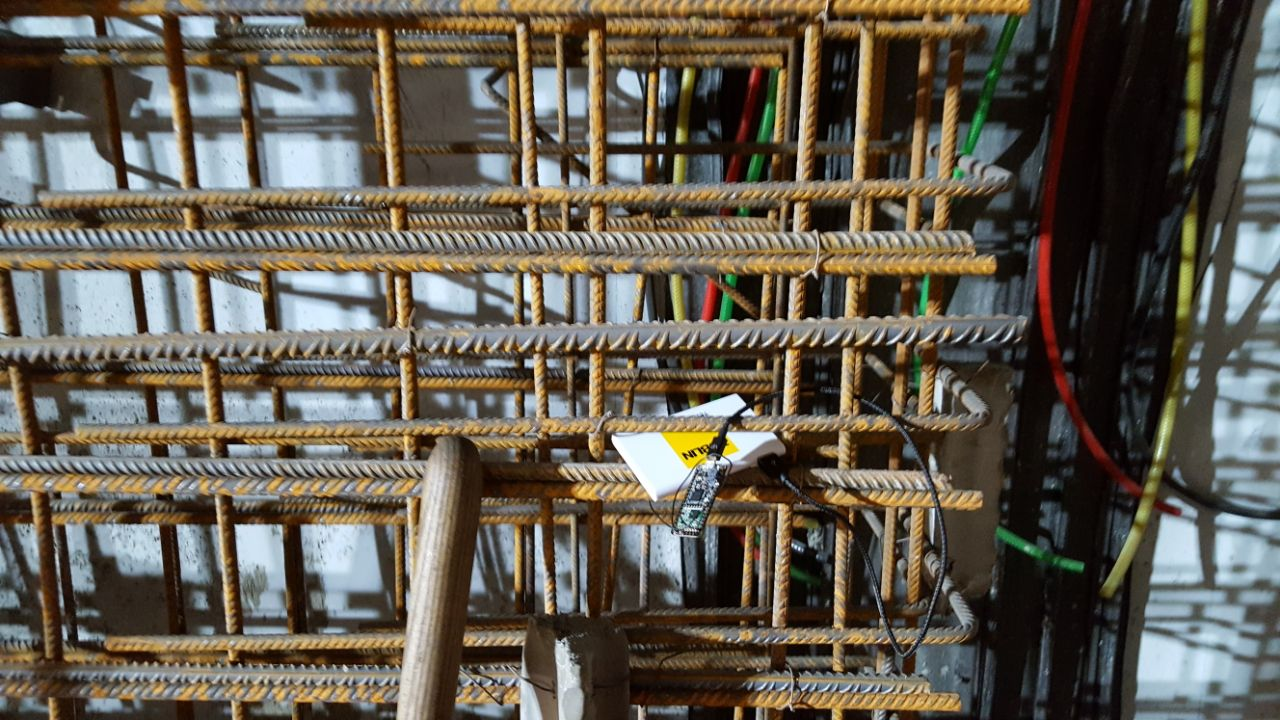
\includegraphics[width=\textwidth]{images/lorabasis.jpg}
  \caption{Platzierung der mobilen Einheit an der Bewehrung des Tunnels.}
  \label{fig:lorabasis}
\end{figure}

\subsection{Ergebnisse}
Tabelle \ref{table:rangelora} zeigt die Ergebnisse für das RFM95.
Da das lose Auflegen des Deckels der Plastikbox zu keiner Veränderung bei der Reichweite führte gibt die Tabelle nur Werte für den offenen Aufbau an. 
Der Test mit 23dBm Sendeleistung durch alle drei Schalungswagen musste nach 350 Metern abgebrochen werden, weil ein weiterkommen nicht möglich war.
Da jedoch für diese Sendeleistung bereits nach circa 250 Metern die Varianz des RSSI den Zusammenhang zwischen Distanz und RSSI überwiegt, kann die tatsächliche Reichweite dieser Sendeleistung nicht ausgenutzt werden.
Für eine sichere Erkennung des 250-Meter-Abschnitts müsste daher alle 500 Meter eine Basisstation aufgestellt werden.

\begin{table}[h]
	\centering
	\caption{Sendereichweite LoRa-basierter mobiler Einheiten}
	\label{table:rangelora}
	\begin{tabular}{p{2.2cm}|p{1.5cm}|p{2.5cm}|p{3.5cm}|p{3cm}}
		Verwendetes Modul & Aufbau & Sendeleistung & Strecke & Maximale Sendereichweite \\
		\hline
		RFM95 & Offen & 5dBm & Wenige Hindernisse & 250m \\
		RFM95 & Offen & 5dBm & Viele Hindernisse & 100m \\
		\hline
		RFM95 & Offen & 23dBm & Wenige Hindernisse & 1250m \\
		RFM95 & Offen & 23dBm & Viele Hindernisse & >350m \\
	\end{tabular}
\end{table}

\subsection{Bewertung}
LoRa entfaltet im Tunnel eine sehr hohe Reichweite und es kann eine lückenlose Überwachung von Personen durchgeführt werden.
Voll nutzen lässt sich diese jedoch nicht, da die Varianz des RSSI den Zusammenhang zwischen Distanz und RSSI schon nach circa 250 Metern überwiegt. 
Hingegen führt eine starke Reduktion der Sendeleistung zu einer mangelden Penetration von Hindernissen.
Daher sollte ein Kompromiss der Sendeleistung geschlossen werden. 
Eine Sendeleistung von 10dBm sollte eine ausreichende Reichweite im Szenario mit vielen Hindernissen bieten.
Alternativ kann die mobile Einheit auch ein Send-Receive Schema umsetzen und von der Basisstation eine dynamisch angepasste Sendeleistung empfangen, die sich nach der Menge der Hindernisse richtet.\\
Wird die Sendeleistung dynamisch so festgelegt, dass einer Reichweite von 250 Metern erreicht wird benötigt ein Mitarbeiter bei 30 km/h 30 Sekunden um sie zu durchqueren.
Eine derart lange Intervallzeit würde jedoch dazu führen, dass eine volle Minute ohne Aktualisierung der Position vergeht, sollte ein Paket verloren gehen.
Das Sendeintervall wird deshalb auf zehn Sekunden gesetzt.

\section{LoRa Implementierung}
Die Implementierung für die Lokalisierung mit LoRa ist sehr simpel.
Die mobile Einheit versendet regelmäßig ein Paket, welches einen Identifikator für die mobile Einheit enthält.
Das Sendeintervall beträgt entsprechend der hohen Reichweite zehn Sekunden.\\
Die Basisstation empfängt durchgehend und bestimmt den RSSI für eingehende Pakete.
Anschließend leitet sie den Identifikator der mobilen Einheit zusammen mit dem RSSI und einer Kennung für die Basisstation an den Ortungsserver weiter.\\
Auf der mobilen Einheit müssen lediglich die Sendefrequenz, die Sendeleistung und der Identifikator gesetzt werden, dann kann immer nach Ablauf des Sendeintervalls gesendet werden.
Die Basisstation muss dabei auf der selben Frequenz aktiv sein und empfangen.


\section{Untersuchung des Energieverbrauchs}
Der Energieverbrauch soll mit dem INA219 genauer bestimmt werden, der INA219 und die verwendete Methodik werden in Abschnitt \ref{ch:phase1:sec:energie} beschrieben.

\subsection{Theoretische Energieverbrauchsabschätzung}
Für die Berechnung des theroretischen Verbrauchs der mobilen Einheit werden die Datenblätter des M0 Mikrocontrollers und des RFM95 Radios herangezogen. 
Die dort gelisteten Verbräuche sind in Tabelle \ref{table:m0power} und Tabelle \ref{table:lorapower} zu finden.

\begin{table}[h]
  \centering
  \caption{Stromverbrauch des M0 Mikrocontrollers, aus \cite{nxp2016m0}}
	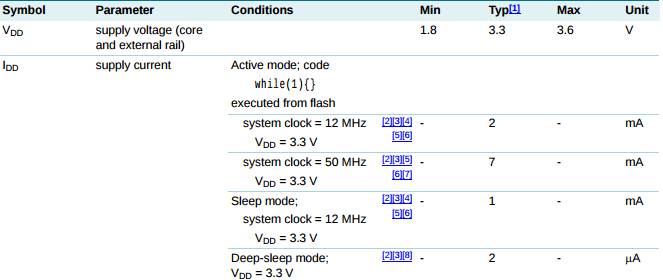
\includegraphics[width=\textwidth]{images/m0power.png}
  \label{table:m0power}
\end{table}

\begin{table}[h]
  \centering
  \caption{Stromverbrauch des RFM95, aus \cite{hope2006rfm}}
	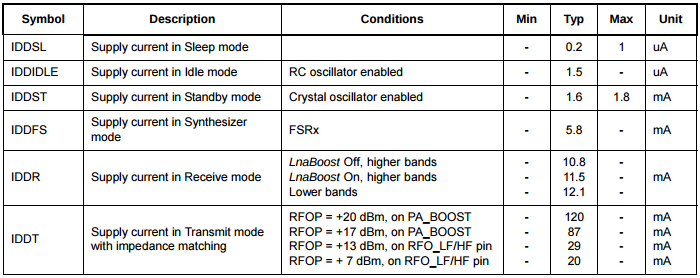
\includegraphics[width=\textwidth]{images/lorapower.png}
  \label{table:lorapower}
\end{table}

Da das Adadfruit Feather M0 RFM95 Lora Radio ansonsten baugleich zum Adafruit Feather nRF52 ist werden die 155 Mikroamper für die sonstigen Komponenten übernommen.\\
Die Sendeleistung des RFM95 Radio ist zwischen 5dBm und 23dBm einstellbar. 
Das Datenblatt listet jedoch nur Verbräuche zwischen 7dBm und 20dBm Sendeleistung, der Verbrauch wird für diese beiden Sendeleistungen berechnet.
Für die Nachricht "{}TagTest"{} werden 20 Bytes (160 Bits) versendet, es wird angenommen, dass zuvor 500 Bits für die Kollisionskontrolle belauscht werden.\\[1cm]

$y = \frac{1}{10} * [(10 - \frac{Bits\_gesendet}{21875 b/s} - \frac{Bits\_empfangen}{21875 b/s}) * (M0\_Deep\_sleep\_mode + RMF95\_IDDIDLE + 155 {\mu}A) + \frac{Bits\_gesendet}{21875 b/s} * RFM95\_XdBm + \frac{Bits\_empfangen}{21875 b/s} * RFM95\_IDDR]$\\[0.5cm]
$y_{20dBm} = \frac{1}{10} * [(10s - 0,0073s - 0,0229s) * 0,1585mA + 0,0073s * 120mA + 0,0229s * 12,1mA]$\\[0.5cm]
$y_{20dBm} \approx \frac{1}{10} * (1,58mA + 0,876mA + 0,2771mA) = 0,2683mA$\\[1cm]

$y_{7dBm} = \frac{1}{10} * [(10s - 0,0073s - 0,0229s) * 0,1585mA + 0,0073s * 20mA + 0,0229s * 12,1mA]$\\[0.5cm]
$y_{7dBm} \approx \frac{1}{10} * (1,58mA + 0,146mA + 0,2771mA) = 0,1953mA$\\[1cm]

\subsection{Tatsächlicher Energieverbrauch von LoRa}
\label{ch:phase3:sec:powerlora}
Der Stromverbrauch der Implementierung mit LoRa wurde mit 5dBm und 23dBm Sendeleistung überprüft
Abbildung \ref{fig:lora23} zeigt den Lastverlauf für den Start einer mobilen Einheit mit LoRA bei 23dBm.\\
Nach einer circa drei sekündigen Startphase wechselt der LoRa Feather in den regulären Betrieb, er sollte dann immer nach zehn Sekunden Ruhezustand senden.
Dieser jedoch vom Zeitgeber nicht ganz eingehalten, die mobile Einheit befindet sich zwischen den Sendevorgängen circa elf Sekunden im Ruhezustand, dies sollte bei der Implementierung beachtet werden.
Im Ruhezustand liegt der Verbrauch des LoRa Feather bei 2,5 bis 2,7 Milliamper, beim Senden unterscheiden sich die Vebräuche je nach Sendeleistung deutlich.\\

\begin{figure}[h!]
  \centering
	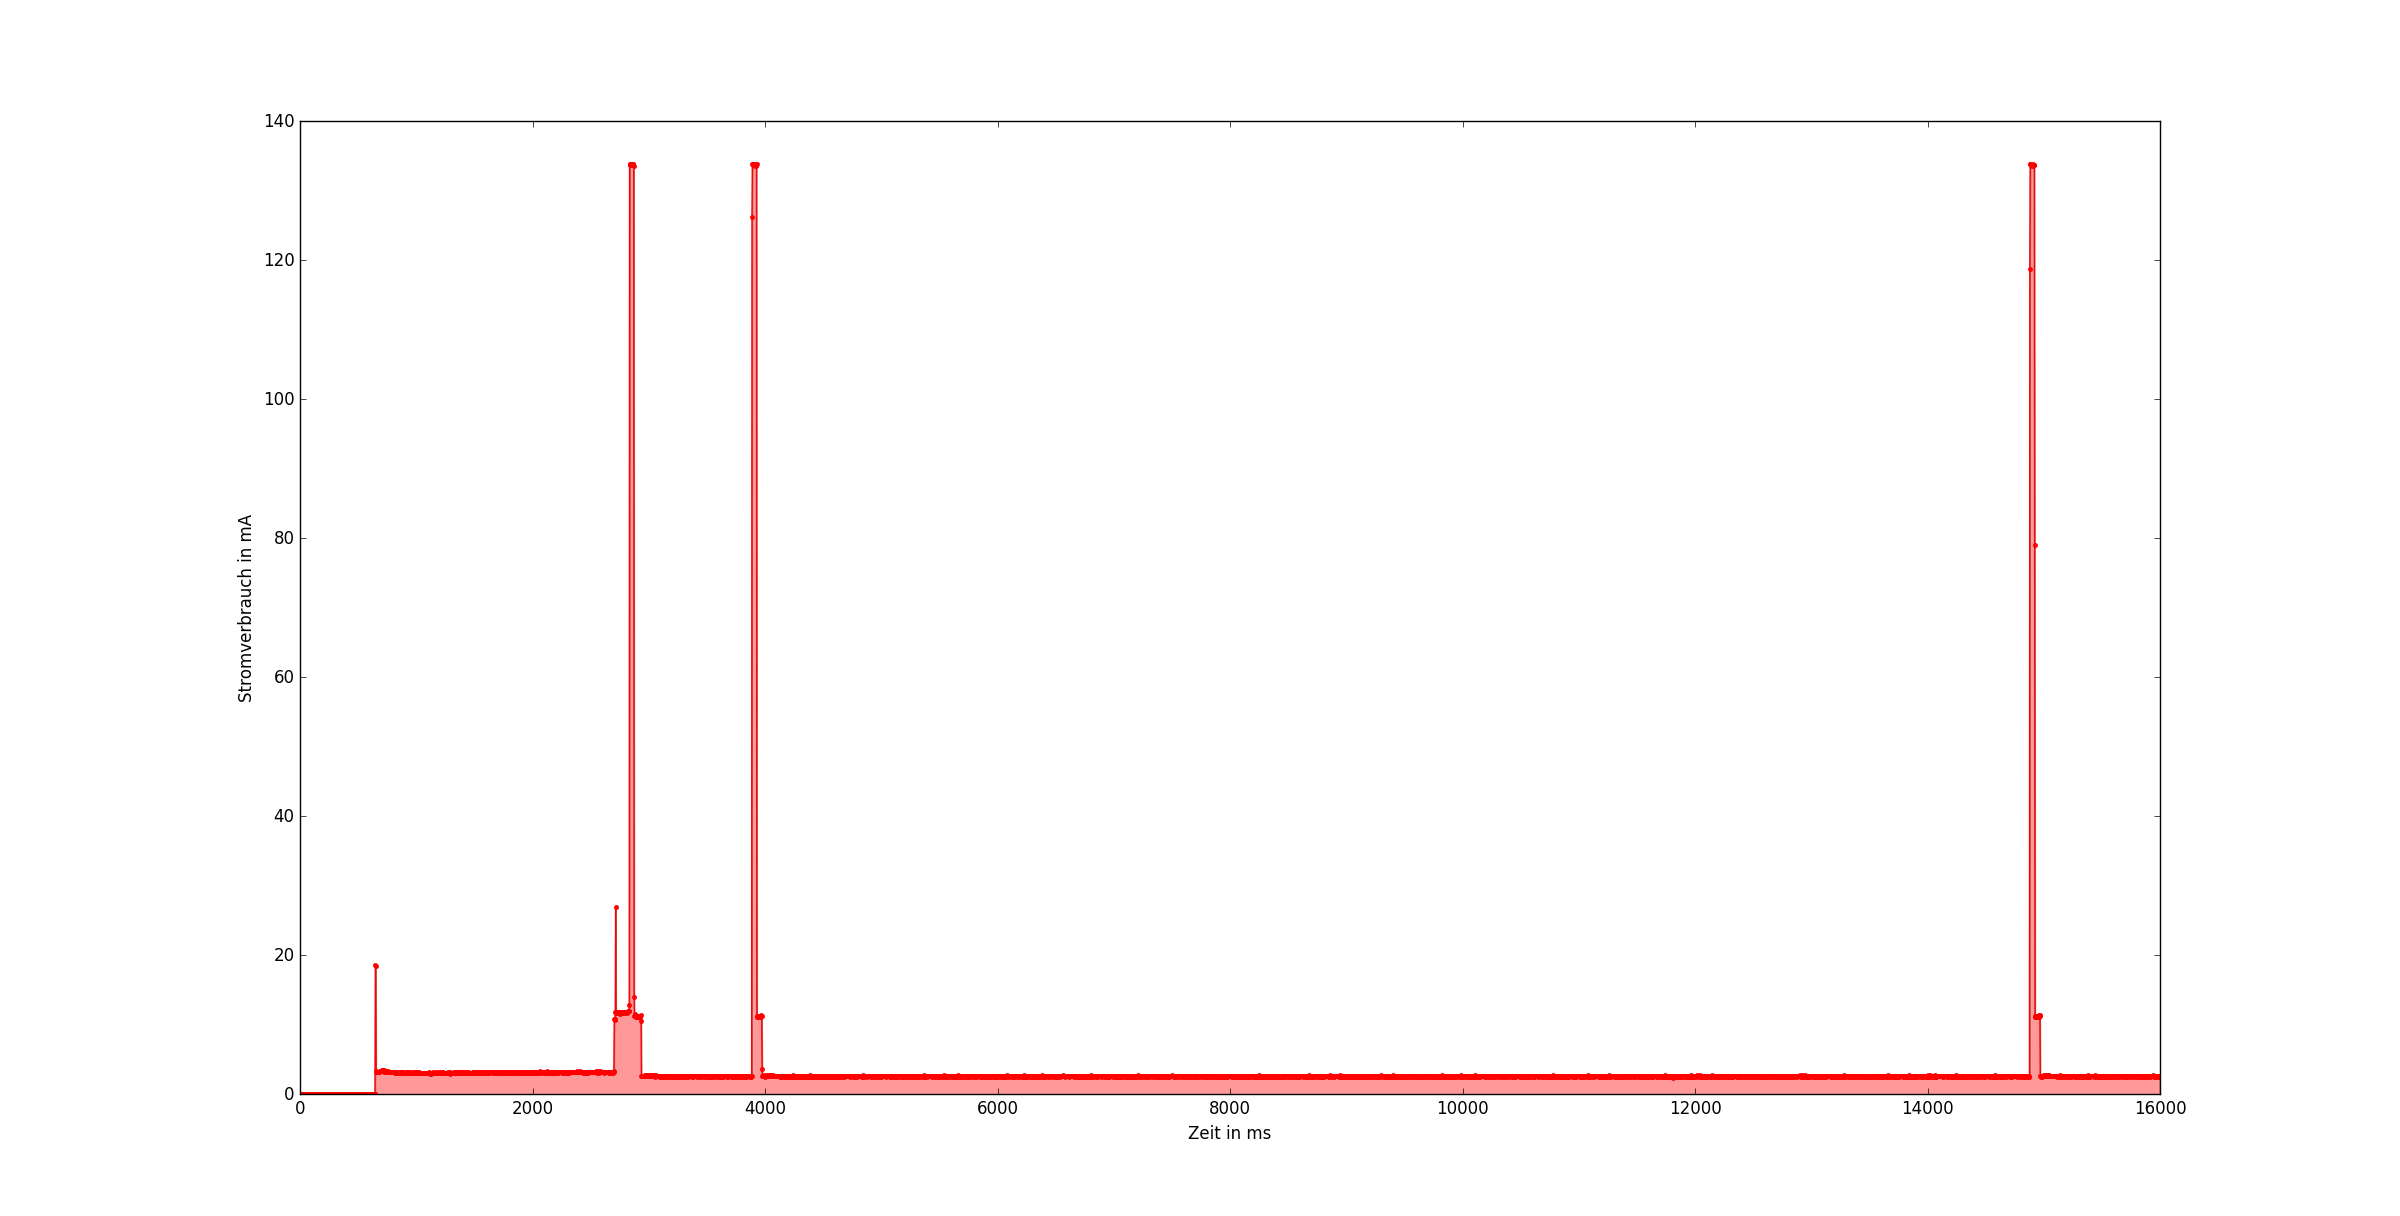
\includegraphics[width=\textwidth]{plots/lora23.png}
  \caption{Lastkurve einer Implementierung mit LoRa.}
  \label{fig:lora23}
\end{figure}

Die Abbildung \ref{fig:lora235send} zeigt die Sendeverbäuche für eine Sendeleistung von 23dBm in Rot und für 5dBm in Grün.
Gut zu erkennen ist hier auch, dass ein Sendevorgang bei LoRa deutlich länger als bei Bluetooth Low Energy dauert, obwohl vergleichbar viele Bits übertragen werden.

\begin{figure}[h!]
  \centering
	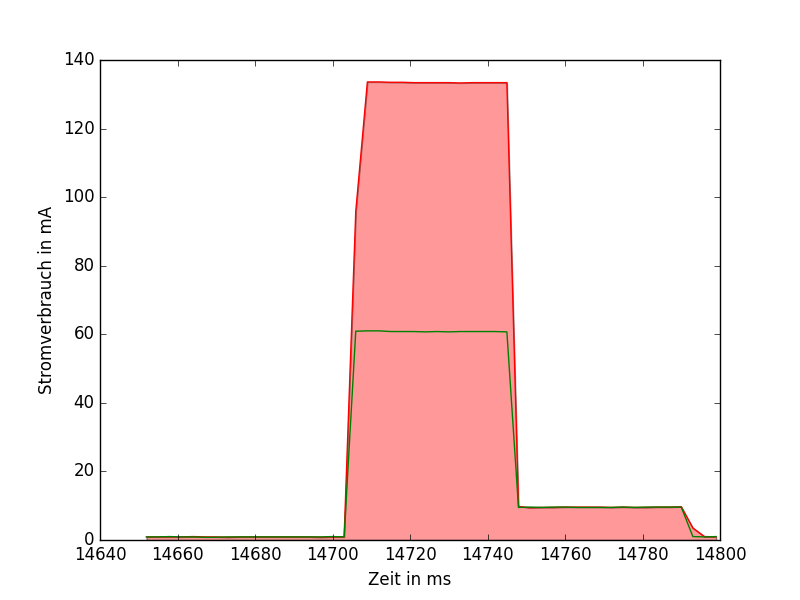
\includegraphics[width=\textwidth]{plots/lora235send.png}
  \caption{Lastkurve eines Ortungsvorgangs mit LoRa.}
  \label{fig:lora235send}
\end{figure}

Die Ergebnisse der Messungen sind in Tabelle \ref{table:lora235ina} gelistet.\\
Für den LoRa Feather liegt der Ruheverbrauch deutlich niedriger, da jedoch die selben Schaltungen für Akku-Ladung und Spannungsregelung zum Einsatz kommen scheint der CP2104, welcher zum Programmieren des ESP8266 beziehungsweise nRF52 dient, mindestens 4,5 Milliamper zu verbrauchen.

\begin{table}[h!]
	\centering
	\caption{Energieverbrauch mobiler Einheiten mit LoRa}
	\label{table:lora235ina}
	\begin{tabular}{p{3.5cm}|p{5cm}|p{2.5cm}|p{2.5cm}}
		Hardware & Programm & $\varnothing$ Verbrauch in mA & Laufzeit in Stunden\\
		\hline
		LoRa Feather & LoRa mit 23dBm Sendeleistung & 3,16 & 443\\
		LoRa Feather & LoRa mit 5dBm Sendeleistung & 2,88 & 486,1\\
	\end{tabular}
\end{table}


